%% This is file `elsarticle-template-5-harv.tex',
%%
%% Copyright 2009 Elsevier Ltd
%%
%% This file is part of the 'Elsarticle Bundle'.
%% ---------------------------------------------
%%
%% It may be distributed under the conditions of the LaTeX Project Public
%% License, either version 1.2 of this license or (at your option) any
%% later version.  The latest version of this license is in
%%    http://www.latex-project.org/lppl.txt
%% and version 1.2 or later is part of all distributions of LaTeX
%% version 1999/12/01 or later.
%%
%% The list of all files belonging to the 'Elsarticle Bundle' is
%% given in the file `manifest.txt'.
%%
%% Template article for Elsevier's document class `elsarticle'
%% with harvard style bibliographic references
%%
%% $Id: elsarticle-template-5-harv.tex 159 2009-10-08 06:08:33Z rishi $
%% $URL: http://lenova.river-valley.com/svn/elsbst/trunk/elsarticle-template-5-harv.tex $
%%
\documentclass[preprint,authoryear,11pt]{elsarticle}

%% Use the option review to obtain double line spacing
%% \documentclass[authoryear,preprint,review,12pt]{elsarticle}

%% Use the options 1p,twocolumn; 3p; 3p,twocolumn; 5p; or 5p,twocolumn
%% for a journal layout:
%%\documentclass[final,authoryear,1p,times]{elsarticle}
%%\documentclass[final,authoryear,1p,times,twocolumn]{elsarticle}
%%\documentclass[final,authoryear,3p,times]{elsarticle}
%%\documentclass[final,authoryear,3p,times,twocolumn]{elsarticle}
%%\documentclass[final,authoryear,5p,times]{elsarticle}
%%\documentclass[final,authoryear,5p,times, twocolumn, 12pt]{elsarticle}


%% if you use PostScript figures in your article
%% use the graphics package for simple commands
%% \usepackage{graphics}
%% or use the graphicx package for more complicated commands
\usepackage[demo]{graphicx}
\graphicspath{ {figura/} }
%% or use the epsfig package if you prefer to use the old commands
%%\usepackage{epsfig}

\usepackage[export]{adjustbox}
\usepackage{float}
\usepackage{dblfloatfix}
\usepackage{lipsum}
\usepackage{multicol}
\setlength{\columnsep}{1cm}
%%\setlength{\columnseprule}{1pt}
%%\usepackage{geometry}
%%\geometry{legalpaper, landscape, margin=2in}
\usepackage[a4paper, total={7in, 9in}]{geometry}
\usepackage[utf8]{inputenc}
\usepackage{url}
\usepackage{hyperref}

%% The amssymb package provides various useful mathematical symbols
\usepackage{amssymb}
%% The amsthm package provides extended theorem environments
%% \usepackage{amsthm}

%% The lineno packages adds line numbers. Start line numbering with
%% \begin{linenumbers}, end it with \end{linenumbers}. Or switch it on
%% for the whole article with \linenumbers after \end{frontmatter}.
%% \usepackage{lineno}

%% natbib.sty is loaded by default. However, natbib options can be
%% provided with \biboptions{...} command. Following options are
%% valid:

%%   round  -  round parentheses are used (default)
%%   square -  square brackets are used   [option]
%%   curly  -  curly braces are used      {option}
%%   angle  -  angle brackets are used    <option>
%%   semicolon  -  multiple citations separated by semi-colon (default)
%%   colon  - same as semicolon, an earlier confusion
%%   comma  -  separated by comma
%%   authoryear - selects author-year citations (default)
%%   numbers-  selects numerical citations
%%   super  -  numerical citations as superscripts
%%   sort   -  sorts multiple citations according to order in ref. list
%%   sort&compress   -  like sort, but also compresses numerical citations
%%   compress - compresses without sorting
%%   longnamesfirst  -  makes first citation full author list
%%
%% \biboptions{longnamesfirst,comma}

% \biboptions{}

%\journal{Nuclear Physics B}
\journal{Computers, Environment and Urban Systems}

\begin{document}

\begin{frontmatter}

%% Title, authors and addresses

%% use the tnoteref command within \title for footnotes;
%% use the tnotetext command for the associated footnote;
%% use the fnref command within \author or \address for footnotes;
%% use the fntext command for the associated footnote;
%% use the corref command within \author for corresponding author footnotes;
%% use the cortext command for the associated footnote;
%% use the ead command for the email address,
%% and the form \ead[url] for the home page:
%%
%% \title{Title\tnoteref{label1}}
%% \tnotetext[label1]{}
%% \author{Name\corref{cor1}\fnref{label2}}
%% \ead{email address}
%% \ead[url]{home page}
%% \fntext[label2]{}
%% \cortext[cor1]{}
%% \address{Address\fnref{label3}}
%% \fntext[label3]{}

%\title{}
\title{Proposta de Infraestrutura de Dados Espaciais para o Setor Elétrico no Brasil\tnoteref{t1}}
\tnotetext[t1]{Artigo para Qualificação de Mestrado no Programa de Pós-Graduação em Geografia}
%% use optional labels to link authors explicitly to addresses:
%% \author[label1,label2]{<author name>}
%% \address[label1]{<address>}
%% \address[label2]{<address>}

%\author{}
\author{Candido, D. S.\corref{cor1}}
\ead{diogosantana@aneel.gov.br}
\ead[url]{sigel.aneel.gov.br}

\author{Carvalho Junior, O. A\corref{cor2}}
\ead{osmarjr@unb.br}

%\address{}
\address{Universidade de Brasília, Instituto de Ciências Humanas, Departamento de Geografia, Brasília, DF - Brasil}


\cortext[cor1]{Aluno de Mestrado}
\cortext[cor2]{Professor Orientador}


\begin{abstract}
%% Text of abstract

\end{abstract}

\begin{keyword}
%% keywords here, in the form: keyword \sep keyword

%% MSC codes here, in the form: \MSC code \sep code
%% or \MSC[2008] code \sep code (2000 is the default)

\end{keyword}

\end{frontmatter}

% \linenumbers
%% main text
%\section{}
\section{Introdução}
\label{sec1}
\begin{multicols}{2}

Com os avanços decorrentes da evolução dos meios de aquisição de dados geoespaciais (ex.: sensoriamento remoto, GPS, aerofotogrametria, conversão de dados geoespaciais analógicos para digitais) e das plataformas dos Sistemas de Informações Geográficas - SIG aliados com o desenvolvimento da Tecnologia da Informação e Comunicação - TIC, proporcionaram a popularização das informações geoespaciais, assim consideradas aquelas que possuem uma dimensão espacial, para servirem de subsídio de conhecimento aos tomadores de decisões nas mais diversas situações, escalas e importância na sociedade \citep{Macharis2014AFlanders, Kounadi2016AdaptiveDatasets, Bejar2012AnInfrastructures, Borzacchiello2013EstimatingE-Cadastres, Hamylton2012DevelopmentSeychelles}. O controle e o gerenciamento dos dados geoespaciais pode ser atribuídos a própria entidade responsável pela produção, manutenção e compartilhamento desses dados, ou por outras entidades que atuem apenas no campo político e administrativo, essa heterogeneidade no controle e gerenciamento prejudica a adequada descrição dos dados no preenchimentos do metadados, situação agravante no âmbito governamental por possui uma grande diversidade de instituições e de dados geoespaciais \citep{Grus2011AnGoals}. Algumas dificuldades surgiram com esse aumento exponencial da produção de dados geoespaciais, podemos citar como as principais, a não existência de padrões definidos e de metodologia para a sua produção, dificultando a interoperabilidade, e a dificuldade do conhecimento da existência dos dados geoespaciais e seu acesso, proporcionando a duplicidade de dados e assim acarretando aumento de custos \citep{concar}. 

As boas práticas relacionadas a gestão dos recursos corporativos tem sido evidenciada e buscada pelas principais entidades governamentais e não governamentais, o conceito de Governo Eletrônico \citep{eping} que pode ser conceituado como iniciativas estatais para facilitar o acesso à informação para a sociedade por meio da Internet, ampliando as discussões sobre a prestação dos serviços públicos com enfoque no aumento da sua efetividade, neste cenário, uma Infraestrutura de Dados Espaciais - IDE apresenta-se, como importante ferramenta para o acesso as informações geoespaciais de forma simples, sem a necessidade de um conhecimento especializado, bastando apenas acesso a Internet para que o usuário comum possa usufruir dessas informações \citep{Borzacchiello2013EstimatingE-Cadastres}.

Assim como para os demais setores da sociedade, o setor elétrico no Brasil abrangendo a geração, transmissão e distribuição de energia elétrica, possui uma crescente demanda por informações geoespaciais, podemos destacar os principais usuários para estas informações, o Ministério de Minas e Energia - MME, instituição responsável pela formulação e supervisão das políticas públicas na área de energia elétrica;   a Agência Nacional de Energia Elétrica - ANEEL, instituição responsável pela regulação e fiscalização dos serviços públicos de energia elétrica; a Empresa de Pesquisa Energética - EPE, instituição responsável pelos estudos e pesquisas para subsidiar o planejamento energético; Eletrobras, instituição responsável pelas operações destinadas ao suprimento de energia elétrica no Brasil; Operador Nacional do Sistema Elétrico - ONS, instituição responsável pela coordenação e controle da operação das instalações de geração e transmissão de energia elétrica no Sistema Interligado Nacional - SIN; Concessionárias, Autorizadas e Permissionárias dos serviços públicos de energia elétrica; Investidores e Empreendedores; e os cidadãos. A evidência desse grande número de usuários e de produtores de informações geoespaciais, demonstra a necessidade e a importância que uma IDE temática para o setor de energia pode subsidiar as tomadas de decisões que possuem como objetivos a melhora dos serviços públicos de energia elétrica e redução de custos na obtenção dessas informações geoespaciais.         



\section{Infraestrutura de Dados Espaciais}

Uma IDE pode ser entendida como um conjunto de políticas, padrões, tecnologias e acordos institucionais para o acesso, compartilhamento, interoperabilidade, organização e disseminação de dados geoespaciais, utilizando uma arquitetura baseada em Geo Serviços disponibilizados pela Internet, permitindo assim o acesso as informações geoespaciais \citep{DAmore2012ICTManagement, Kobben2013TowardsInfrastructure, Stock2012ToInfrastructure, Hendriks2012ReconsideringInfrastructure, NeamahJebur2013ANSDI, Makanga2010AAfrica}. As IDEs pode ser classificadas quanto ao tipo de escala de implementação em Global (ex.: \citeauthor{unggim}), Continental (ex.: \citeauthor{inspire}), Nacional (ex.: \citeauthor{inde,nsdi,cgdi}), Institucional (ex.: \citeauthor{geoportal}) ou Departamental, essa escolha vai depender basicamente do seu público alvo e do tipo de informação \citep{Bejar2012AnInfrastructures}, e quanto ao enfoque a IDE pode ser num primeiro nível mais corporativo abrangendo os acordos institucionais, definição de políticas, normais e regulamentação para a sua implementação nas instituições, ocupando um nível mais estratégico e num segundo nível mais técnico abrangendo definições e especificações dos serviços de mapas e protocolos web, modelagem de dados e catálogos de metadados, neste caso ocupando um nível mais operacional \citep{Cooper2013AViewpoint}. 

\subsection{Infraestrutura Nacional de Dados Espaciais no Brasil}
\label{sec2}
O Decreto de número 6.666 de 2008 do Poder Executivo Federal, considerado o Marco Legal da IDE do Brasil, regulamentou a Infraestrutura Nacional de Dados Espaciais - INDE e a implantação do Diretório Brasileiro de Dados Geoespaciais (\citeauthor{dbdg}), que deverá utilizar o Portal Brasileiro de Dados Geoespaciais, denominado “Sistema de Informações Geográficas do Brasil - SIG Brasil”, como o portal principal para o acesso aos dados geoespaciais, seus metadados e  os Geo Serviços relacionados \citep{d6666}. A Comissão Nacional de Cartografia - CONCAR, órgão colegiado do Ministério do Planejamento, Orçamento e Gestão - MPOG responsável pelo Plano de Ação para Implantação da INDE \citep{concar}, compõem-se do Conselho Superior ocupando um nível mais estratégico para a implantação da INDE com as definições de políticas e normas, e também existe para subsidiar as ações da CONCAR, o Comitê Técnico e os Grupos de Trabalhos ocupando um nível mais operacional da INDE. Quanto as Normas, Padrões e Especificações Técnicas do Sistema Cartográfico Nacional - SCN estabelecidas para a INDE, o Exército Brasileiro - EB através da Diretoria de Serviços Geográfico - DSG responde pelo mapeamento sistemático com as escalas de 1:250.000 e maiores, o Instituto Brasileiro de Geografia e Estatística - IBGE responde pela rede geodésica fundamental e pelo mapeamento sistemático das escalas menores de 1:250.000, a Marinha do Brasil - MB através da Diretoria de Hidrografia e Navegação - DHN pelas cartas náuticas de qualquer escala e a Aeronáutica através do Instituto de Cartografia Aeronáutica -ICA  pelas cartas aeronáuticas de qualquer escala \citep{dl243}.    

Ainda no decreto que regulamentou a INDE, foram definidos os seguintes objetivos nas esferas federal, estadual, distrital e municipal: Promover o ordenamento da geração, armazenamento, acesso, compartilhamento, disseminação e uso dos dados geoespaciais; promover a utilização dos padrões e normas homologadas pela CONCAR; e evitar a duplicidade de ações e desperdiço de recursos públicos na obtenção de dados geoespaciais \citep{d6666}. 

A INDE tem como base os seguintes documentos para a suas definições de regras e padrões, assim como para a sua fundamentação teórica: especificações técnicas para a Estruturação de Dados Geoespaciais Vetoriais - EDGV \citep{edgv}, para a Aquisição de Dados Geoespaciais Vetoriais - ADGV \citep{adgv}, dos Produtos de Conjuntos de Dados Geoespaciais - PCDG \citep{pcdg}, para a Representação de Dados Geoespaciais - RDG \citep{mt347001,mt347002}, para o Controle de Qualidade dos Produtos de Conjuntos de Dados Geoespaciais - CQPCDG \citep{cqpcdg}, do Perfil de Metadados Geoespaciais do Brasil - Perfil MGB \citep{pmgb}, dos Padrões de Interoperabilidade Governo Eletrônico - ePING \citep{eping} e da Open Geospatial Consortium - OGC \citep{ogc}. A Mapoteca Nacional Digital - MND criada para a disponibilização dos mapeamentos sistemáticos dos diversos órgãos que respondem pelo SCN, pode ser subdividida em 3 componentes, a estruturação vetorial, matricial e a de metadados. Com relação a componente vetorial, as especificações técnicas da ADGV para a aquisição da geometria dos dados geoespaciais e a EDGV para a modelagem conceitual destinam-se especialmente aos desenvolvedores e usuários de SIG, dentro da modelagem conceitual dos dados geoespaciais as classes de objetos são agrupados nas seguintes categorias de informações: Abastecimento de Água e Saneamento Básico, Administração Pública, Educação e Cultura, Energia e Comunicações, Estrutura Econômica, Hidrografia, Limites, Localidades, Pontos de Referência, Relevo, Saúde e Serviço Social, Sistemas de Transportes e Vegetação \citep{edgv}. Este artigo propõe a complementação da categoria Energia e Comunicação com uma abordagem mais temática específica para os usuários do setor de energia do Brasil. 

\subsection{Infraestrutura de Dados Espaciais no Setor Elétrico}
\label{sec3}

A já enfatizada importância de uma IDE temática para o setor de energia no Brasil devido a sua pluralidade de atores produzindo e utilizando os dados geoespaciais, também possui a CONCAR como o órgão principal para estabelecer os padrões de uma IDE temática do setor de energia de forma que assegure a sua compatibilidade com o que está prescrito na INDE. No que concerne quais classes de objetos que vão ser incluídas nessa modelagem conceitual temática e como elas se relacionarão, cabe aos usuários em geral atuantes no setor de energia elétrica estabelecer.       

\section{Metodologia para implantar uma Infraestrutura de Dados Espaciais}
\label{sec4}

Uma IDE busca facilitar o acesso as informações geoespaciais de forma que elas sejam altamente interoperáveis, a arquitetural ideal para essas funcionalidades trata-se da Arquitetura Orientada a Serviços - AOS utilizando os serviços web baseados em padrões simples e não proprietários para a comunicação e o intercâmbio de dados geoespaciais. Os principais elementos utilizados são os dados geoespaciais, metadados desses dados e os geo serviços web, assim podemos dividir a arquitetura de uma IDE na Camada de Dados, que contém os dados geoespaciais e os metadados associados a esses dados, na Camada de Serviços em que os dados geoespaciais e os metadados são publicados em geo serviços e a Camada de aplicação onde os geo serviços obedecem aos padrões e protocolos web para seu acesso via Internet \citep{Kobben2013TowardsInfrastructure,Li2011Semantic-basedInfrastructure,Miro2010MetadataSystems}.
Escrever: Descrever a modelagem conceitual/banco de dados, GeoServiços do Setor Elétrico, Portal de Geoprocessamento.
\end{multicols}

\begin{figure}[H]
    \centering
    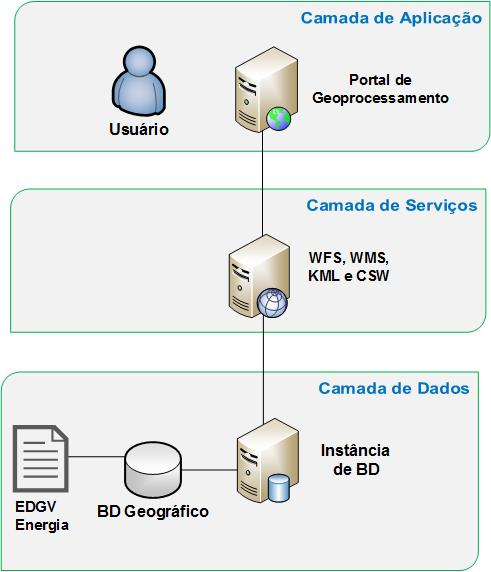
\includegraphics[scale=0.7]{fig3}
    \caption{Arquitetura IDE Energia}
    \label{fig:my_label}
\end{figure}


\section{Resultados}
\label{sec5}
\begin{multicols}{2}
\end{multicols}

\begin{figure}[H]
\centering
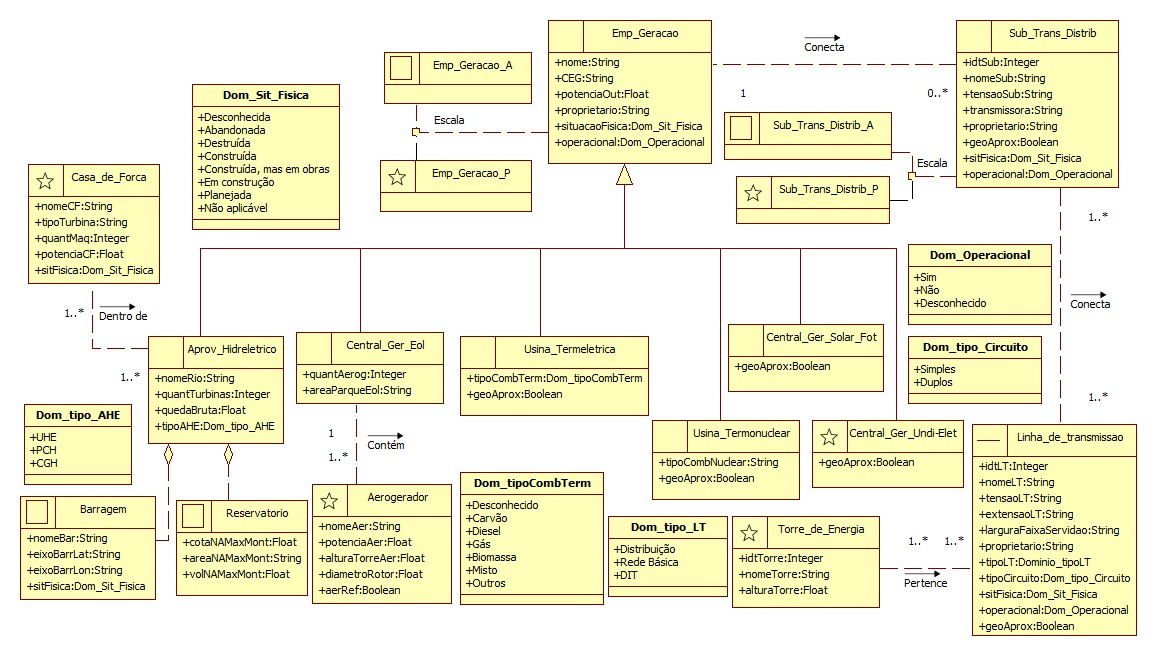
\includegraphics[scale=0.8,angle=90]{fig} 
\caption{Modelagem Conceitual do Tema Energia}
\label{fig:subim1}
\end{figure}

\begin{multicols}{2}

\section{Discussão}
\label{sec6}
Texto

\section{Conclusão}
\label{sec7}
Texto

\appendix
\section{Descrição dos atributos}
\label{appendix}

\end{multicols}

"Tabela com a Descrição dos Atributos"

%% The Appendices part is started with the command \appendix;
%% appendix sections are then done as normal sections
%% \appendix

%% \section{}
%% \label{}

%% References
%%
%% Following citation commands can be used in the body text:
%%
%%  \citet{key}  ==>>  Jones et al. (1990)
%%  \citep{key}  ==>>  (Jones et al., 1990)
%%
%% Multiple citations as normal:
%% \citep{key1,key2}         ==>> (Jones et al., 1990; Smith, 1989)
%%                            or  (Jones et al., 1990, 1991)
%%                            or  (Jones et al., 1990a,b)
%% \cite{key} is the equivalent of \citet{key} in author-year mode
%%
%% Full author lists may be forced with \citet* or \citep*, e.g.
%%   \citep*{key}            ==>> (Jones, Baker, and Williams, 1990)
%%
%% Optional notes as:
%%   \citep[chap. 2]{key}    ==>> (Jones et al., 1990, chap. 2)
%%   \citep[e.g.,][]{key}    ==>> (e.g., Jones et al., 1990)
%%   \citep[see][pg. 34]{key}==>> (see Jones et al., 1990, pg. 34)
%%  (Note: in standard LaTeX, only one note is allowed, after the ref.
%%   Here, one note is like the standard, two make pre- and post-notes.)
%%
%%   \citealt{key}          ==>> Jones et al. 1990
%%   \citealt*{key}         ==>> Jones, Baker, and Williams 1990
%%   \citealp{key}          ==>> Jones et al., 1990
%%   \citealp*{key}         ==>> Jones, Baker, and Williams, 1990
%%
%% Additional citation possibilities
%%   \citeauthor{key}       ==>> Jones et al.
%%   \citeauthor*{key}      ==>> Jones, Baker, and Williams
%%   \citeyear{key}         ==>> 1990
%%   \citeyearpar{key}      ==>> (1990)
%%   \citetext{priv. comm.} ==>> (priv. comm.)
%%   \citenum{key}          ==>> 11 [non-superscripted]
%% Note: full author lists depends on whether the bib style supports them;
%%       if not, the abbreviated list is printed even when full requested.
%%
%% For names like della Robbia at the start of a sentence, use
%%   \Citet{dRob98}         ==>> Della Robbia (1998)
%%   \Citep{dRob98}         ==>> (Della Robbia, 1998)
%%   \Citeauthor{dRob98}    ==>> Della Robbia

\begin{multicols}{2}
%% References with bibTeX database:
\bibliographystyle{model5-names}
%%\bibliography{mendeley}
\bibliography{sample}

%% Authors are advised to submit their bibtex database files. They are
%% requested to list a bibtex style file in the manuscript if they do
%% not want to use model5-names.bst.

%% References without bibTeX database:

% \begin{thebibliography}{00}

%% \bibitem must have one of the following forms:
%%   \bibitem[Jones et al.(1990)]{key}...
%%   \bibitem[Jones et al.(1990)Jones, Baker, and Williams]{key}...
%%   \bibitem[Jones et al., 1990]{key}...
%%   \bibitem[\protect\citeauthoryear{Jones, Baker, and Williams}{Jones
%%       et al.}{1990}]{key}...
%%   \bibitem[\protect\citeauthoryear{Jones et al.}{1990}]{key}...
%%   \bibitem[\protect\astroncite{Jones et al.}{1990}]{key}...
%%   \bibitem[\protect\citename{Jones et al., }1990]{key}...
%%   \harvarditem[Jones et al.]{Jones, Baker, and Williams}{1990}{key}...
%%

% \bibitem[ ()]{}

% \end{thebibliography}
\end{multicols}
\end{document}

%%
%% End of file `elsarticle-template-5-harv.tex'.
